\section{Materiais Refratários Monolíticos}\label{mono}

	Os materiais refratários são componentes fundamentais nas economias modernas exercendo o papel de indústria habilitadora no sentido que possibilita a execução de processos a elevadas solicitações térmicas, químicas e mecânicas em um ambiente controlado e seguro. Ademais, o contexto sócio-ambiental do século XXI exige o máximo cuidado a fim de reduzir o desperdício de energia, especialmente de processos que ocorrem a altas temperaturas, onde a perda de energia para o ambiente é inerente.

	Assim, a indústria de materiais refratários está diretamente ligada a outras indústrias fundamentais como a indústria de cimento e principalmente a siderúrgica, ambas indústrias extremamente correlacionadas com o produto interno bruto (PIB) das nações, conforme demonstrado no gráfico temporal mostrado na Figura \ref{fig:refractory_economy}

\begin{figure}[ht]
\centering
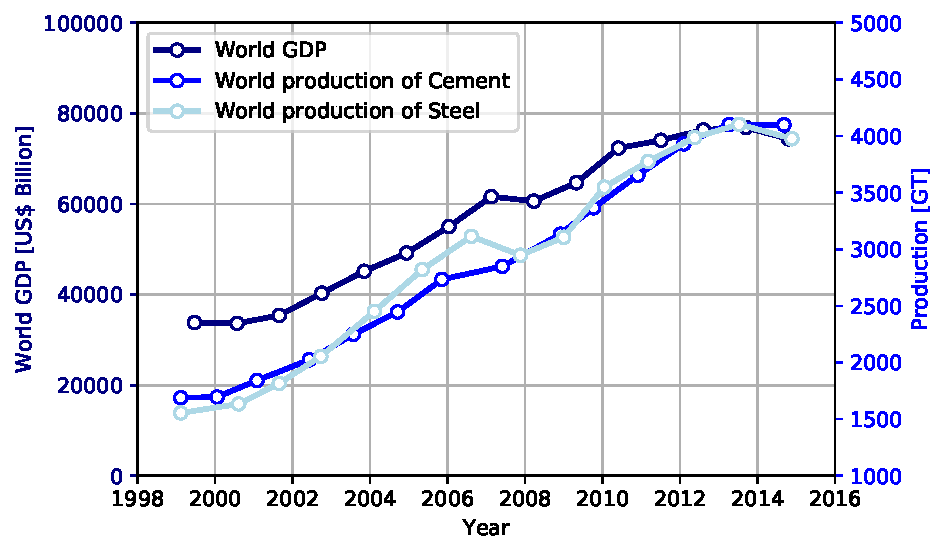
\includegraphics[width=\linewidth]{./figures/refractory_economy.pdf}
\caption{Evolução temporal do PIB mundial (azul escuro, eixo esquerdo), da produção mundial de Aço e Cimento (azul e azul claro, eixo direito) no período de 1999 a 2015.  Adaptado de \cite{GlobalRef2017}. \label{fig:refractory_economy}}
\end{figure}
		Com esse papel fundamental, os materiais refratários (que também passam por processos em alta temperatura durante sua fabricação) também passam por uma mudança de paradigma relativamente recente, isto é, ao invés do produtor fornecer peças pré-formadas (refratários conformados), este passa a oferecer um material conformável (monolítico), o que otimiza a logística - do ponto de vista do produtor, evita e reduz estoques, reduz o custo energético e permite uma maior customização do produto por parte do comprador.
        Dessarte, a seguir é realizada uma breve revisão do conceito de materiais monolíticos explorando seu processamento e finalmente vantagens e desvantagens características de tal classe de materiais.

    \subsection{Conceito}
      Capítulos 10 e 11 - Livro Ana
    

    \subsection{Processamento}
      Capítulos 10 e 11 - Livro Ana


    \subsection{Vantagens e desvantagens}
      Capítulos 10 e 11 - Livro Ana